\subsection{Seismic Inversion}

In this experiment we perform an inversion of a seismic survey line using a
one-dimensional seismic sensor forward model. The goal is to infer both the
geometry of the interfaces between subsurface geological layers and the
seismic propagation velocity within each layer from noisy surface observations
of the sound reflection times, \Outs. 
% We use two datasets for this experiment; a simulated
%world with two randomly generated splines representing geological layers (providing a ground-truth), 
Our dataset is part of a real interpreted (specifying reflection time
estimates rather than raw sound waves) seismic survey from the Otway basin in
South Australia.  It contains a line of 113 sites over the Pretty Hill region,
providing reflection times for the four shallowest layer formations.
% Each dataset has 50 and 113 observations per layer respectively.

The inputs, $\Ins$, are the surface locations (metres) of the seismic sensors,
and we use the following forward model,
\begin{align}
    \latents_p^\text{depth} &= \max\cbrac{\latents_p^\text{depth, input},
        \latents_{p-1}^\text{depth}} \quad \forall p, \label{eq:clip} \\
    \nonlinf_p^\text{time} &=
    \begin{cases}
        2\frac{\latents_p^\text{depth} - \latents_{p-1}^\text{depth}}
        {\latents_p^\text{vel}} + \nonlinf_{p-1}^\text{time},
        & \text{if } p > 0 \\
        2\frac{\latents_0^\text{depth}}{\latents_0^\text{vel}},
        & \text{if } p = 0
    \end{cases}
\end{align}
Where there are $\otdim$ output tasks -- reflection times from each layer,
$\nonlinf_p^\text{time}$, and there are two types of latent input tasks;
\begin{itemize}
    \item $\latents_p^\text{depth}\!\brac{\Ins}$, the geological depth of layer
        $p$ corresponding to each surface location. Equation \eqref{eq:clip} 
        clips overlapping estimated (input) layers to create these valid
        layers.
    \item $\latents_p^\text{vel}\!\brac{\Ins}$, the velocity of layer $p$ 
        below each surface input location.
\end{itemize}

Naturally, we wish to infer both the depth and velocity of four layers below
each survey site. Likewise $\ltdim = 2\otdim$, and the problem is
under-constrained since there is an infinite set of layer depths and
velocities that can generate the reflection times. To help constrain our
models, we center the latent function priors on average depths and velocities
of each layer.

%We compare against two baseline methods. The first baseline applies
%gradient-free optimisation to identify the maximum a-posteriori latent tasks.
%A GMRF prior is used to model the deviation of each layer from a flat mean
%function.

A baseline probabilistic approach using MCMC has been implemented to sample from
the posterior distribution. To make the problem more managable for the sampling-based baseline method, 
the dimensionality of the 
MCMC problem has been reduced by parameterising each latent task with $20$ 
regularly spaced radial basis functions (truncated cosine), such that the MCMC
learns the distribution of their weights. In addition to the weights, an 
observation noise variance parameter was introduced for each of the four 
observed taks. Independent Gaussian priors are placed on the basis weights, and 
a Gamma prior on each of the per-task observation variances.

The EKS and UKS methods were applied to the same problem, using an equivalent 
prior on the weight space.
%We adapted the MCMC 
%prior by projecting our learned basis weights into the space of the radial 
%basis functions, and used the same prior on per-task observation variances. 
The results of both the EKS and UKS methods were very similar. Figure 
\ref{fig:seismic_result} shows the results from the EKS method inferring the 
distribution over layer boundary depths (top) and seismic transmission 
velocities (bottom). Draws from the above MCMC baseline are overlaid. Clearly
the MCMC draws are in agreement with the structure of the layer velocities and 
depths. However, we do note that the MCMC draws are smoother. This may be 
because the limited number of radial basis functions used in the MCMC has 
restricted the ability of the baseline MCMC to infer high frequency details.

\begin{figure}
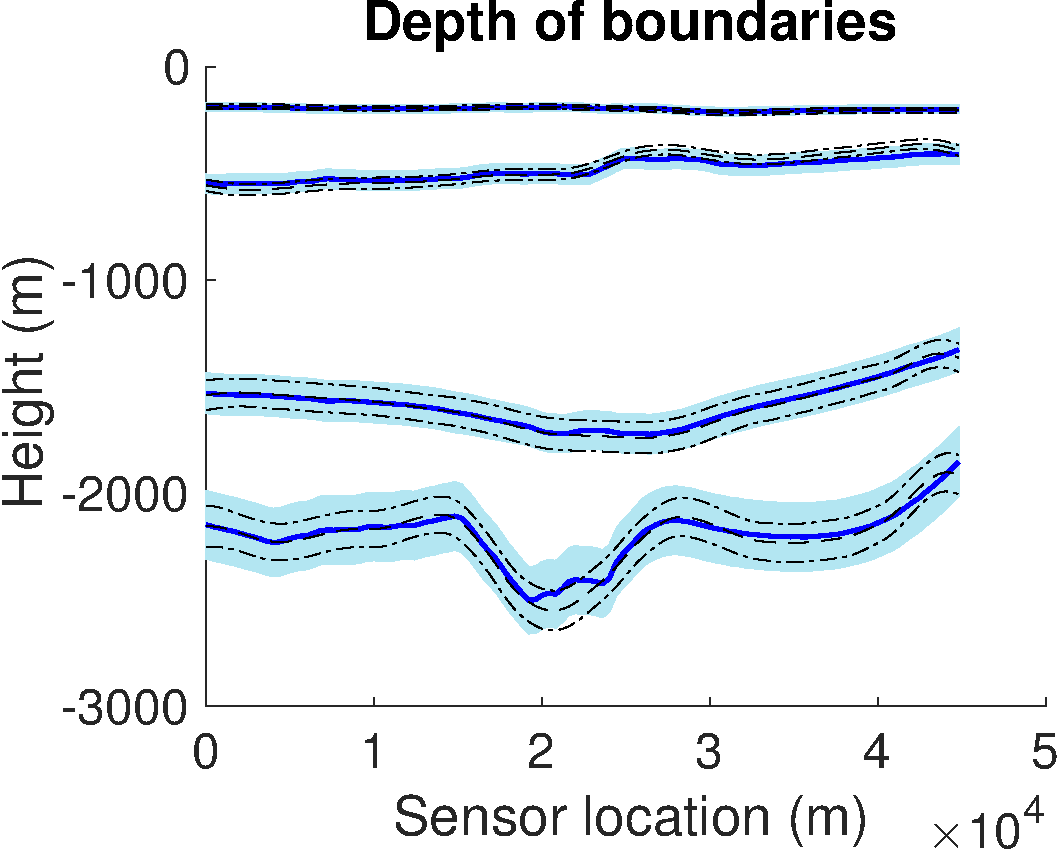
\includegraphics[width=0.4\textwidth]{seismicData-depth-Taylor-1000} \\
\includegraphics[width=0.4\textwidth]{seismicData-vel-Taylor-1000}
\caption{Results of the EKS on the seismic inversion problem. The inferred 
    layer boundaries (top) and seismic velocities (bottom) are shown in blue, 
    indicating the predictive means and 3 standard deviation envelopes. Draws
    from the MCMC inversion are overlaid in dotted black.}
 \label{fig:seismic_result}
\end{figure}

